\begin{section}[]{\uppercase{Results and Discussion}}
 \addtocontents{toc}{\uppercase{Results and Discussion}}

 \subsection{Training Factors A}
 After augumentation of the data, the model was trained for 20 epochs with a train generator and validation generator, resulting in good model accuracy for each model. 
 The training factors have been summarized in the table \ref{tab:training_factors}.

 \begin{table}[htbp]
    \centering
    \begin{tabular}{ll}
        \toprule
        \textbf{Training factor} & \textbf{Values} \\
        \midrule
        Platform & Google Colaboratory \\
        TPU & Python 3 Google Compute Engine backend \\
        Optimizer & Adam \\
        Loss function & Categorical cross-entropy \\
        Learning rate & 0.001 \\
        Epoch & 20 \\
        Batch size & 10 \\
        \bottomrule
    \end{tabular}
    \caption{List of materials and tools used for training the model}
    \label{tab:training_factors}
\end{table}


\subsubsection{Training and Validation Results}

The table below presents the training and validation loss and accuracy metrics for each epoch during the training process of the dual-input Convolutional Neural Network (CNN) model. The training was conducted over 20 epochs. The performance metrics demonstrate the following key observations:

\begin{itemize}
    \item \textbf{Training Accuracy:} The training accuracy exhibits a high starting point at approximately 90.27\% in the first epoch, stabilizing around 85-90\% in subsequent epochs. This indicates the model's consistent learning pattern.
    \item \textbf{Validation Accuracy:} The validation accuracy is remarkably high, starting at 98.31\% in the first epoch and achieving a perfect accuracy of 100\% in the 18th epoch. The consistently high validation accuracy suggests that the model generalizes well to unseen data.
    \item \textbf{Training Loss:} The training loss shows fluctuations throughout the epochs, starting at 0.3247 and reaching 0.1859 by the 20th epoch. This variability could indicate the model's ongoing adjustments during the learning process.
    \item \textbf{Validation Loss:} The validation loss demonstrates significant variability, with values ranging from 0.0036 to 0.2476. The lowest validation loss occurs in the 18th epoch, at 0.0036, corresponding to the highest validation accuracy.
\end{itemize}

These results underscore the model's high performance and generalization capabilities. The low validation loss in several epochs highlights the model's effectiveness in minimizing error on unseen data, whereas the variability in training loss suggests continuous learning and optimization during training.

\begin{table}[htbp]
    \centering
    \begin{tabular}{llllll}
    \toprule
    \textbf{Epoch} & \textbf{Training Loss} & \textbf{Training Accuracy} & \textbf{Validation Loss} & \textbf{Validation Accuracy} \\ 
    \midrule
    1  & 0.3247 & 0.9027 & 0.0354 & 0.9831 \\ 
    \midrule
    2  & 0.2831 & 0.8749 & 0.0755 & 0.9746 \\ 
    \midrule
    3  & 0.3369 & 0.8315 & 0.2476 & 1.0000 \\ 
    \midrule
    4  & 0.3365 & 0.8627 & 0.0219 & 0.9915 \\ 
    \midrule
    5  & 0.2225 & 0.8766 & 0.2333 & 0.9153 \\ 
    \midrule
    6  & 0.3035 & 0.8401 & 0.0577 & 0.9661 \\ 
    \midrule
    7  & 0.2589 & 0.8532 & 0.0219 & 0.9915 \\ 
    \midrule
    8  & 0.2451 & 0.8636 & 0.0958 & 0.9492 \\ 
    \midrule
    9  & 0.1923 & 0.8871 & 0.0184 & 0.9915 \\ 
    \midrule
    10 & 0.2542 & 0.8566 & 0.0231 & 0.9831 \\ 
    \midrule
    11 & 0.2476 & 0.8610 & 0.0102 & 0.9915 \\ 
    \midrule
    12 & 0.2438 & 0.8471 & 0.0354 & 0.9831 \\ 
    \midrule
    13 & 0.2718 & 0.8514 & 0.1603 & 0.8898 \\ 
    \midrule
    14 & 0.2670 & 0.8332 & 0.0903 & 0.9576 \\ 
    \midrule
    15 & 0.2376 & 0.8784 & 0.0242 & 0.9831 \\ 
    \midrule
    16 & 0.2470 & 0.8566 & 0.0181 & 0.9915 \\ 
    \midrule
    17 & 0.1699 & 0.8454 & 0.0117 & 0.9915 \\ 
    \midrule
    18 & 0.1808 & 0.8766 & 0.0036 & 1.0000 \\ 
    \midrule
    19 & 0.2671 & 0.8714 & 0.0322 & 0.9915 \\ 
    \midrule
    20 & 0.1859 & 0.8940 & 0.0207 & 0.9915 \\ 
    \bottomrule
    \end{tabular}
    \caption{Epoch-wise Training and Validation Results for Adam Optimizer}
    \label{table:results-a}
    \end{table}
 
\begin{figure}[H]
    \centering
    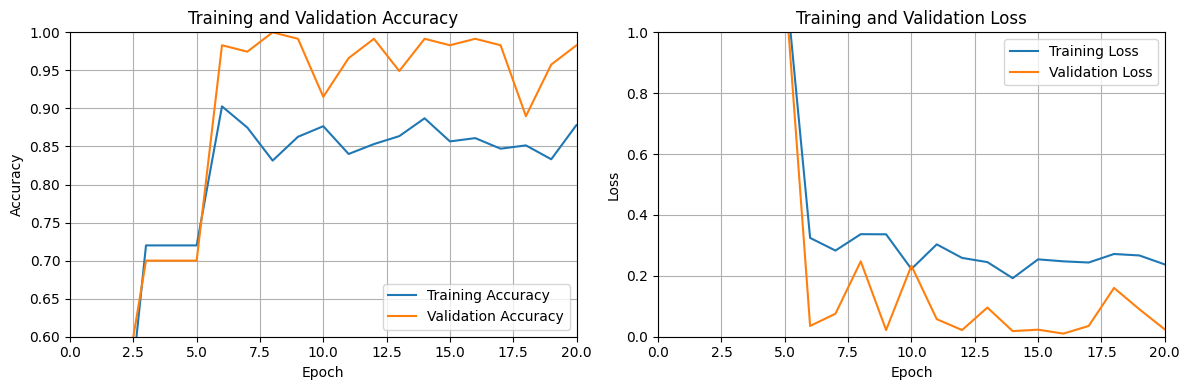
\includegraphics[width=\linewidth]{images/result.png}
    \caption{Training and Validation Results for Adam Optimizer}
    \label{fig:result}
\end{figure}

\subsection{Training Factors B}
The model was compiled with RMSProp optimizer and categorical cross-entropy loss function. RMSProp (Root Mean Square Propagation) is an optimization algorithm that uses the moving average of the squared gradient to normalize the gradient. It is an adaptive learning rate method that divides the learning rate by the moving average of the squared gradient. This helps to adjust the learning rate based on the gradient's magnitude, making it more stable and efficient.
The training factors have been summarized in the table \ref{tab:training_factors_b}.
\begin{table}[H]
    \centering
    \begin{tabular}{ll}
        \toprule
        \textbf{Training factor} & \textbf{Values} \\
        \midrule
        Platform & Google Colaboratory \\
        TPU & Python 3 Google Compute Engine backend \\
        Optimizer & RMSProp \\
        Loss function & Categorical cross-entropy \\
        Learning rate & 0.001 \\
        Epoch & 20 \\
        Batch size & 10 \\
        \bottomrule
    \end{tabular}
    \caption{List of materials and tools used for training the model}
    \label{tab:training_factors_b}
\end{table}



\subsubsection{Training and Validation Results}

The table below presents the training and validation loss and accuracy metrics for each epoch.
\begin{itemize}
    \item \textbf{Training Accuracy}: The training accuracy starts at approximately 77.76\% in the first epoch and shows a general upward trend, reaching 94.70\% by the 20th epoch. This indicates that the model is effectively learning and improving its performance.
    \item \textbf{Validation Accuracy}: The validation accuracy starts at a high 94.92\% in the first epoch, achieving perfect accuracy (100\%) in several epochs, including the second and final epochs. This suggests strong generalization ability to unseen data.
    \item \textbf{Training Loss}: The training loss starts high at 36.7045 in the first epoch but decreases significantly over the epochs, indicating the model's improved ability to minimize error during training.
    \item \textbf{Validation Loss}: The validation loss exhibits fluctuations, starting at 0.3475 in the first epoch, reaching as low as 0.0007 in the second epoch, and ending at 0.0063 in the final epoch. The low validation loss in multiple epochs highlights the model's effectiveness.
\end{itemize}

\begin{table}[H]
\centering
\begin{tabular}{llllll}
\toprule
\textbf{Epoch} & \textbf{Training Loss} & \textbf{Training Accuracy} & \textbf{Validation Loss} & \textbf{Validation Accuracy} \\ 
\midrule
    1  & 36.7045 & 0.7776 & 0.3475 & 0.9492 \\ 
    \midrule
    2  & 2.3207  & 0.8888 & 0.0007 & 1.0000 \\ 
    \midrule
    3  & 1.0619  & 0.9079 & 2.5053 & 0.8136 \\ 
    \midrule
    4  & 0.8817  & 0.9123 & 0.2394 & 0.9068 \\ 
    \midrule
    5  & 0.7055  & 0.9331 & 0.1060 & 0.9746 \\ 
    \midrule
    6  & 0.9905  & 0.9209 & 0.0614 & 0.9746 \\ 
    \midrule
    7  & 0.7818  & 0.9357 & 0.2718 & 0.9661 \\ 
    \midrule
    8  & 0.4616  & 0.9288 & 0.0055 & 1.0000 \\ 
    \midrule
    9  & 0.3379  & 0.9348 & 0.0353 & 0.9831 \\ 
    \midrule
    10 & 1.2596  & 0.8871 & 0.0474 & 0.9915 \\ 
    \midrule
    11 & 0.3767  & 0.9453 & 0.0691 & 0.9915 \\ 
    \midrule
    12 & 0.3609  & 0.9409 & 0.1279 & 0.9746 \\ 
    \midrule
    13 & 0.8072  & 0.9070 & 0.0652 & 0.9831 \\ 
    \midrule
    14 & 0.3556  & 0.9322 & 0.0606 & 0.9746 \\ 
    \midrule
    15 & 0.6149  & 0.9253 & 0.0292 & 0.9915 \\ 
    \midrule
    16 & 0.4864  & 0.9288 & 0.0336 & 0.9746 \\ 
    \midrule
    17 & 0.5084  & 0.9331 & 0.0493 & 0.9661 \\ 
    \midrule
    18 & 0.3350  & 0.9513 & 0.0325 & 0.9746 \\ 
    \midrule
    19 & 0.3296  & 0.9288 & 0.1307 & 0.9068 \\ 
    \midrule
    20 & 0.1756  & 0.9470 & 0.0063 & 1.0000 \\ 
\bottomrule
\end{tabular}
\caption{Epoch-wise Training and Validation Metrics for RMSProp Optimizer}
\label{table:results-b}
\end{table}

\begin{figure}[H]
    \centering
    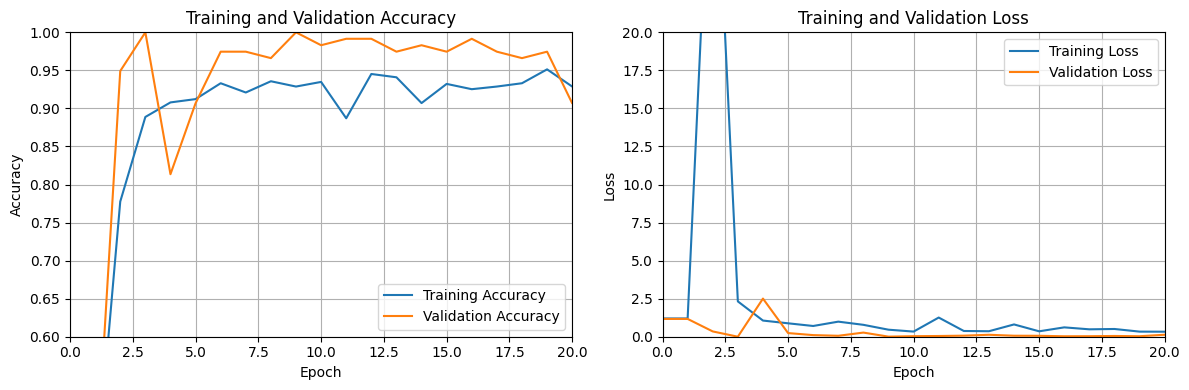
\includegraphics[width=\linewidth]{images/result-2.png}
    \caption{Training and Validation Results for RMSProp Optimizer}
    \label{fig:result-2}
\end{figure}

\subsection{Discussion}
\subsubsection{Performance Validation with XAI}
To analyze the deefake, it is crucial to identify real from fakes and that the model is not biased. SHAP was employed in the base paper, whereas LIME was added to the research to provide more explanation.
The Local Interpretable Model-Agnostic Explanations (LIME) algorithm was applied to the proposed
model. The LIME algorithm is a popular XAI algorithm that can be used to explain image samples with
visual representation. LIME is a model-agnostic algorithm that approximates the local linear behavior of the model.
LIME helps us understand why the model made a particular decision by showing which parts of the image were important.
The highlighted regions are crucial for the model's prediction. For a real image, these are the areas that convinced the model it is real. For a fake image, these are the areas that convinced the model it is fake.
This helps humans understand the model's decision-making process, making it more transparent and trustworthy.

%arrance lime-fake.png and lime-real.png in 2 columns
\begin{figure}[H]
    \centering
    \begin{minipage}{0.45\textwidth}
        \centering
        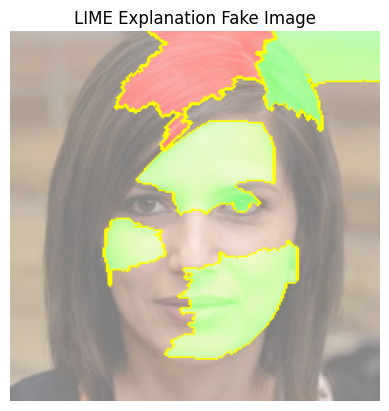
\includegraphics[width=\linewidth]{images/lime-fake.png}
        \captionsetup{font=small}
        \caption{LIME Explanation for Fake Image}
        \label{fig:lime-fake}
    \end{minipage}
    \hfill
    \begin{minipage}{0.45\textwidth}
        \centering
        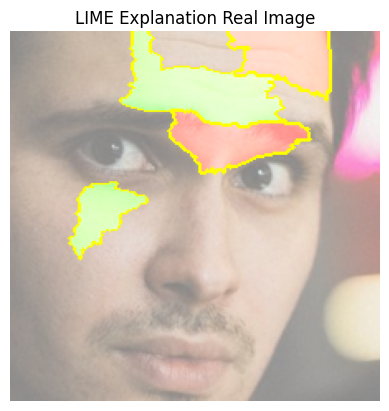
\includegraphics[width=\linewidth]{images/lime-real.png}
        \captionsetup{font=small}
        \caption{LIME Explanation for Real Image}
        \label{fig:lime-real}
    \end{minipage}
\end{figure}



\end{section}

\pagebreak
